\documentclass{article}
\usepackage[final]{neurips_2023}

\usepackage[utf8]{inputenc} % allow utf-8 input
\usepackage[T1]{fontenc}    % use 8-bit T1 fonts
\usepackage{hyperref}       % hyperlinks
\usepackage{url}            % simple URL typesetting
\usepackage{booktabs}       % professional-quality tables
\usepackage{amsfonts}       % blackboard math symbols
\usepackage{nicefrac}       % compact symbols for 1/2, etc.
\usepackage{microtype}      % microtypography
\usepackage{xcolor}         % colors
\usepackage{graphicx}
\usepackage{subfig}
\usepackage{listings}
\usepackage{mathtools}
\usepackage{amsmath}
\usepackage{algorithm}
\usepackage{algpseudocode}

\title{Playing Pokemon Red on GameBoy with PyBoy using Proximal Policy Optimization}


\author{
	Domonkos Kertész\\
	Reinforcement Learning\\
	DM887\\
  	University of Southern Denmark\\
  	\texttt{doker24@student.sdu.dk}}


\begin{document}


\maketitle


\begin{abstract}
	The goal of my project is to apply Proximal Policy Optimization, on parallel running,
	vectorized environments, built upon the library PyBoy.
\end{abstract}


\section{Description}


	The goal of my project is to apply Proximal Policy Optimization, on parallel running,
	vectorized environments, built upon the library PyBoy. The project itself can be found on my GitHub
	\url{https://github.com/KihiraLove/ReinforcementLearning/tree/main/PokemonRedPPO}.
	
\subsection{Development Steps}
	\begin{enumerate}
		\item Setting up additional data files for the game
		\item Setting up PyBoy to load the game and additional files, with the correct configuration
		\item Wrap the PyBoy in a custom Environment that inherits OpenAIs Gym Env
		\item Vectorize the environments with Gymnasium
		\item Implement PPO
		\item Implement additional functions to process result data
	\end{enumerate}

\section{The Environment}
	The environment is based on the Python library clled PyBoy, a GameBoy emulator, that lets me interract with the emulated game, using python. The game in question, PokemonRed, comes from an original GameBoy cartridge, which it was copied from, and was saved into a .gb file. This file is passed to the emulator to run. 

	
	During run my code can interract with the game using the PyBoy API, which lets me use the 6 buttons, that can be used to interract with the game ({\bf A, B, LEFT, UP, RIGHT, DOWN}) and get the current screen from the emulator. While the game itself is continous, the program only observes the screen every 24 frames. This screen data is the aggregated with the last 2 screen data, and auxiliary data (namely the current hitpoints, total level, and exploration progress) as visual status bars, as it can be seen on Figure 1-3, to form a simple short term memory, this data is the fed to the PPO algorithm.


	The way to get information from the game without having to process data from the screen, is to read it from the memory. The memory of PokemonRed is statically allocated, and the game has been reverse engineered, so the memory addresses for the specific data my program needs can be found online.


	The game requires a save file, we either need to supply it with one, or it will automatically create one.


	The emulator is then wrapped by the environment class, that inherits from the Env class of OpenAIs Gymnasium. This way my environment functions the same as a Gym environment would. This way the enviroments can easily be vectorized by Gymnasiums {\tt SyncVectorEnv()} function.

\begin{figure}%
    \centering
    \subfloat[\centering Emulator screen]{{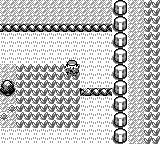
\includegraphics[height=4cm]{exploring_full} }}%
    \qquad
    \subfloat[\centering The algorithms input]{{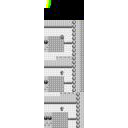
\includegraphics[height=4cm]{exploring_small} }}%
    \caption{The algorithm exploring the map}%
    \label{fig:exploration}%

    \centering
    \subfloat[\centering Emulator screen]{{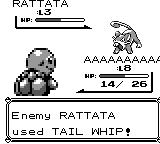
\includegraphics[height=4cm]{battle_full} }}%
    \qquad
    \subfloat[\centering The algorithms input]{{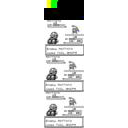
\includegraphics[height=4cm]{battle_small} }}%
    \caption{The algorithm battling with pokémon}%
    \label{fig:battle}%

    \centering
    \subfloat[\centering Emulator screen]{{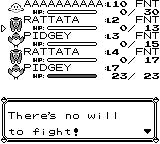
\includegraphics[height=4cm]{menu_full} }}%
    \qquad
    \subfloat[\centering The algorithms input]{{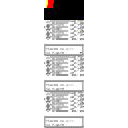
\includegraphics[height=4cm]{menu_small} }}%
    \caption{The algorithm interracting with menus}%
    \label{fig:menu}%
\end{figure}

\subsection{Reward Structure}
	The game itself is complex, it includes an interractable environment, interractable non-player characters, navigatable menus, different screens (overworld, battle), that all needs to be used in combination to progree the game, and reach the goal state. Therefore the reward stucture is required to be quite complex as well, the rewards can be seen on Table 1. On the figure, {\it n} is the rewards scale, which is 1 by default.

The algorithm can score rewards by exploring the map, this is done by comparing the current screen with the previous screen, and if the difference is great enough, reward is given to the algorithm. Other ways to obtain rewards are, participating in events, these are rare unique occasions in the game, catching new pokémon and leveling up pokémon, healing pokémon (replenishing health points after battle), fighting opponents, and receiving badges, which are handed out after beating certain opponents.


\begin{table}
  \caption{Reward Structure}
  \label{reward-table}
  \centering
  \begin{tabular}{lll}
    \toprule
    Name     & Amount     & Description \\
    \midrule
    Event & 4n & Number of events participated in\\
    Level & 4n & Level of gathered pokémons\\
    Heal & 4n & Total healing amount\\
    Opponent Level & 4n & Largest enemy level\\
    Badge & 20n & Number of gathered badges\\
    Explore & 1n & Number of new screens discovered\\
    \bottomrule
  \end{tabular}
\end{table}

\subsection{Start and Goal state}
	The game has a tutorial, which is quite simple for human players.
	\begin{enumerate}
		\item Input player name
		\item Interract with NPCs (non-player characters)
		\item Chose starting pokémon
		\item Travel between two locations to bring an item to an NPC
	\end{enumerate}
	However, these tasks would require either hardcoding certain steps, or modifying the reward structure. To avoid teaching the algorithm a quite linear sequence of events, I have opted to use a save file, {\tt has\_pokedex\_nballs.state}, this is a save file which is loaded for every episode as starting point, where the player has already finished the tutorial, has a starter pokémon, and a small number of pokéballs, which are used throughout the game.


	Similarly, the game is technically endless, the story ends at some point, but the game is playable after. Reaching the ending is a complex goal, which would require thousands of hours of training, therefore I opted to chose an arbitrary ending, which is to obtain the first badge, altough the algorithm never managed to reach this goal.

\section{Proximal Policy Optimization}
	Since OpenAI released it's paper on PPO in 2017, it has became one of the most popular reinforcement learning algorithm, and for good reason, as PPO is a reliable and efficient method for training policies on complex environments, such as mine.

\subsection{Concept}
	
	PPO is a policy based method, where the objective is $\pi(a \mid s; \theta)$, where {\tt s} are states, that are mapped to {\tt a} actions, parameterized by {\tt\(\theta\)}. It optimizes a surrogate objective function that approximates the true objective of maximizing expected cumulative rewards. This objective function includes a ratio between the new policy and the old policy. One of the main innovations in PPO is the introduction of a clipping mechanism in the objective function. The clipped objective ensures that the new policy does not deviate too much from the old policy, thereby preventing large updates that can destabilize training. The clipped objective is given by:

\begin{equation}
L^{\text{CLIP}}(\theta) = \mathbb{E}_t \left[ \min \left( \frac{\pi_\theta(a_t | s_t)}{\pi_{\theta_{\text{old}}}(a_t | s_t)} A_t, \, \text{clip} \left( \frac{\pi_\theta(a_t | s_t)}{\pi_{\theta_{\text{old}}}(a_t | s_t)}, 1 - \epsilon, 1 + \epsilon \right) A_t \right) \right]
\end{equation}

Where $\pi_\theta(a_t \mid s_t)$ is the new policy, $\pi_{\theta_{\text{old}}}(a_t \mid s_t)$ is the old policy.

$A_t$ is the advantage function, and $\epsilon$ is the hyperparameter that controls the clipping range.
The advantage function
\begin{equation}
A_t = Q(s_t, a_t) - V(s_t)
\end{equation}
where:
\begin{itemize}
    \item \( Q(s_t, a_t) \) is the action-value function, representing the expected return for taking action \( a_t \) in state \( s_t \).
    \item \( V(s_t) \) is the value function, representing the expected return for being in state \( s_t \).
\end{itemize}

\subsection{Steps of PPO}

\begin{itemize}
	\item Interact with the environment to collect a set of trajectories (state-action-reward sequences) using the current policy.
	\item Compute the returns (cumulative rewards) for each trajectory and compute the advantages using the value function to reduce variance.
	\item Perform multiple epochs of optimization on the collected data and use the clipped surrogate objective to update the policy parameters, ensuring the updates are not too large.
	\item Simultaneously, update the value function to improve the baseline estimation.
\end{itemize}

\subsection{Pseudocode}

\begin{algorithm}
\caption{Proximal Policy Optimization (PPO)}
\begin{algorithmic}[1]
\State Initialize policy network $\pi_\theta$ and value network $V_\theta$ with random weights
\For{iteration $= 1, 2, \ldots, N$}
    \State Collect trajectories by running policy $\pi_\theta$ in the environment
    \State Compute rewards-to-go (returns) and advantages for each timestep
    \For{epoch $= 1, 2, \ldots, K$}
        \For{each mini-batch of data}
            \State Compute the surrogate loss $L^{\text{CLIP}}(\theta)$
            \State Compute the value function loss
            \State Optimize the policy network using the surrogate loss
            \State Optimize the value network using the value function loss
        \EndFor
    \EndFor
\EndFor
\end{algorithmic}
\end{algorithm}

\subsection{Advantages of PPO}

The pseudocode for Proximal Policy Optimization (PPO) outlines a structured approach to training reinforcement learning agents.

Initially, the policy network $\pi_\theta$ and value network $V_\theta$ are initialized with random weights. The algorithm operates over multiple iterations, where in each iteration, trajectories (sequences of states, actions, and rewards) are collected by executing the current policy in the environment.

Following trajectory collection, the rewards-to-go (returns) and advantages for each timestep are computed to evaluate the quality of actions taken.

The policy and value networks are then optimized over several epochs. During each epoch, the data is divided into mini-batches, and for each mini-batch, the surrogate loss $L^{\text{CLIP}}(\theta)$ is calculated to update the policy network.

This loss function incorporates a clipping mechanism to prevent large updates that could destabilize training.

The value function loss is computed and used to optimize the value network, enhancing its ability to estimate future rewards. This iterative process continues, progressively improving the policy and value networks to achieve better performance in the environment.


\section{Results}
	While the implemented algorithm and environment are quite unstable, and training requires a lot more time and computational resources, than I originally tought it would, I was able to gather some results by running smaller experiments.

	The scale my misjudgement of the training time and resources is severe, solving this task would require thousands of hours of training even on a server with many processor cores, therefore my results training with limited time and on a personal computer, are quite humble. But the algorithm showed progrees, even if small, completed tasks and obtained rewards, better in each episode.
\begin{figure}%
    \centering
    \subfloat[\centering Rewards over 350 episodes]{{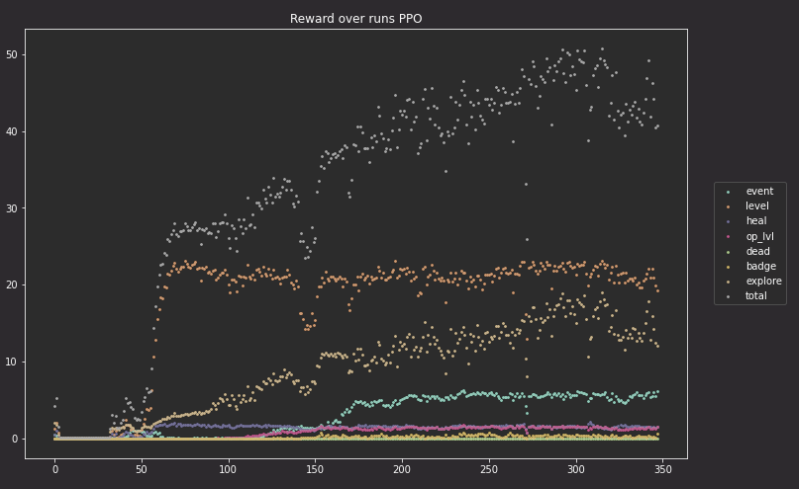
\includegraphics[height=8cm]{Rewards_over_runs} }}%
    \label{fig:rewards-over-runs}%
\end{figure}

\begin{figure}%
    \centering
    \subfloat[\centering Early in training]{{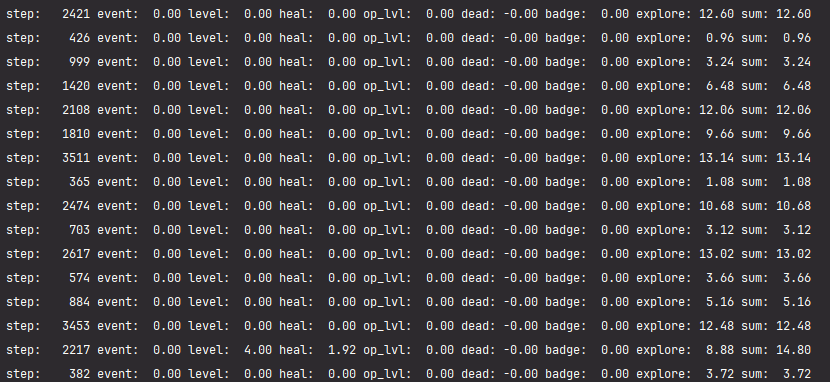
\includegraphics[height=4cm]{rewards} }}%
    \subfloat[\centering Later in training]{{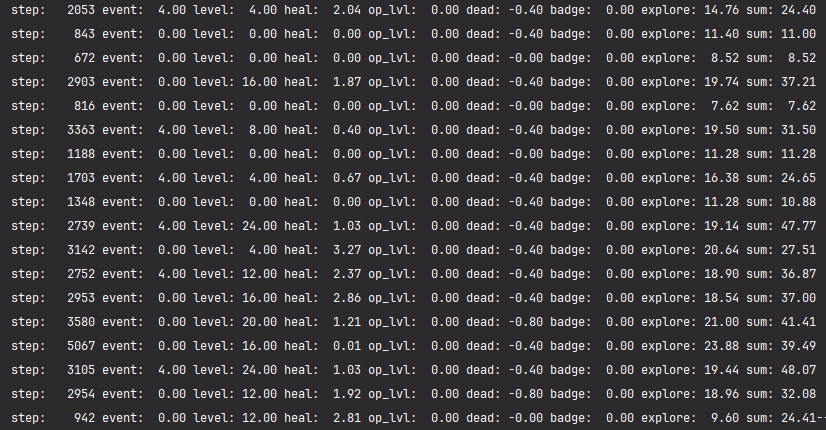
\includegraphics[height=4cm]{rewards2} }}%
    \caption{Collected rewards during training}%
    \label{fig:rewards}%
\end{figure}

\begin{figure}%
    \centering
    \subfloat[\centering Early in training]{{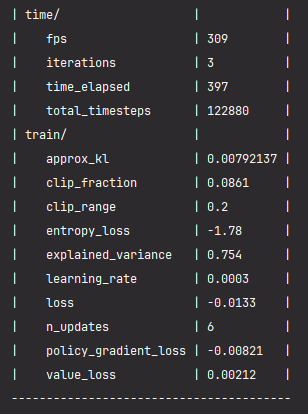
\includegraphics[height=6cm]{stats} }}%
    \qquad
    \subfloat[\centering Later in training]{{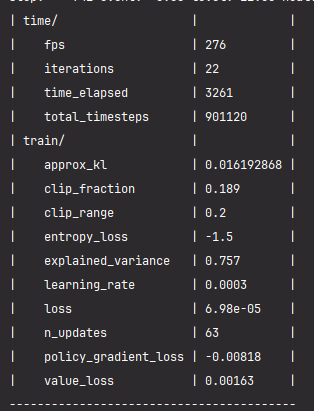
\includegraphics[height=6cm]{stats2} }}%
    \caption{Stats of the training}%
    \label{fig:training-stats}%
\end{figure}

\section{Conclusion}
	This task would require much better resources and more time, but I am personally happy with what I have achieved.
\end{document}